\newpage
\section{Lecture 2: From Shallow to Deep Neural Networks}

\subsection{Supervised Learning Recap}
We mostly work with supervised learning:
\[
\mathcal{D}=\{(\mathbf{x}_i,y_i)\}_{i=1}^{I},
\]
and we train a model that predicts
\[
\hat{y}_i = f(\mathbf{x}_i;\boldsymbol{\phi}).
\]
The training objective is a loss over the dataset:
\[
L(\mathcal{D},\boldsymbol{\phi}) = L(\boldsymbol{\phi}).
\]

\subsection{Shallow Neural Network (One Hidden Layer)}
For 1D input, a shallow ReLU network can be written as
\[
f(x;\boldsymbol{\phi}) = \phi_0 + \sum_{d=1}^{D}\phi_d h_d,
\qquad
h_d = a(\theta_{d0}+\theta_{d1}x),
\]
with ReLU activation
\[
a(z)=\max(z,0).
\]

\newpage

\subsection{Three Activation-Related Graphs}
\begin{figure}[h!]
\centering
\begin{tikzpicture}[scale=0.9]
    % Axes
    \draw[->] (-2.3,0) -- (2.5,0) node[right] {$z$};
    \draw[->] (0,-0.5) -- (0,3.0) node[above] {$a(z)$};
    % Line: a(z) = psi0 + psi1 z = z
    \draw[thick,blue] (-2,-2) -- (2,2);
    \node[blue] at (1.1,2.4) {\scriptsize $a(z)=\psi_0+\psi_1 z,\ \psi_0=0,\psi_1=1$};
\end{tikzpicture}
\hspace{0.6cm}
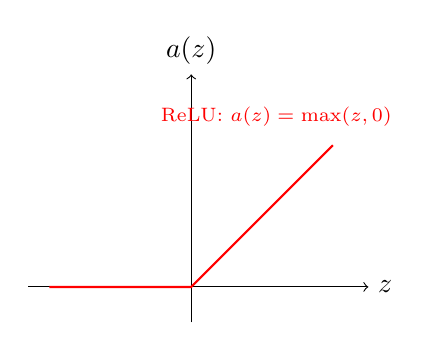
\begin{tikzpicture}[scale=0.9]
    % Axes
    \draw[->] (-2.3,0) -- (2.5,0) node[right] {$z$};
    \draw[->] (0,-0.5) -- (0,3.0) node[above] {$a(z)$};
    % ReLU
    \draw[thick,red] (-2,0) -- (0,0) -- (2,2);
    \node[red] at (1.2,2.4) {\scriptsize ReLU: $a(z)=\max(z,0)$};
\end{tikzpicture}
\hspace{0.6cm}
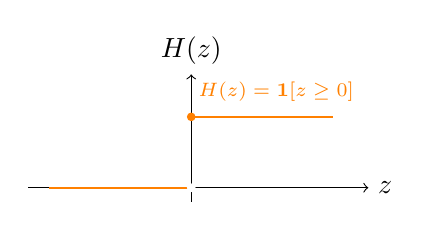
\begin{tikzpicture}[scale=0.9]
    % Axes
    \draw[->] (-2.3,0) -- (2.5,0) node[right] {$z$};
    \draw[->] (0,-0.2) -- (0,1.6) node[above] {$H(z)$};
    % Heaviside
    \draw[thick,orange] (-2,0) -- (0,0);
    \draw[thick,orange] (0,1) -- (2,1);
    \filldraw[white] (0,0) circle (1.5pt);
    \filldraw[orange] (0,1) circle (1.5pt);
    \node[orange] at (1.2,1.35) {\scriptsize $H(z)=\mathbf{1}[z\ge0]$};
\end{tikzpicture}
\caption{Left: linear activation. Middle: ReLU. Right: Heaviside step used in perceptron-style classifiers.}
\end{figure}

\subsection{Perceptron, XOR, and Why Hidden Units Matter}
A single linear perceptron creates one decision boundary, so XOR cannot be solved
with one linear unit. With hidden units and gradient-based learning, we can represent XOR.

For the specific construction:
\[
h_1 = a(0+x_1+x_2),\qquad
h_2 = a(-1+x_1+x_2),\qquad
y = 0+h_1-2h_2.
\]

\begin{figure}[h!]
\centering
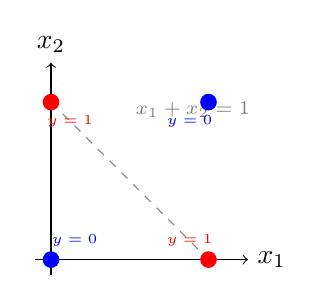
\begin{tikzpicture}[scale=2.0]
    % Axes
    \draw[->] (-0.1,0) -- (1.25,0) node[right] {$x_1$};
    \draw[->] (0,-0.1) -- (0,1.25) node[above] {$x_2$};

    % Linear boundaries x1+x2=0 and x1+x2=1
    \draw[dashed] (0,0) -- (0.05,-0.05);
    \draw[dashed,gray] (0,1) -- (1,0);
    \node[gray] at (0.9,0.95) {\scriptsize $x_1+x_2=1$};

    % XOR points
    \filldraw[blue] (0,0) circle (1.4pt);
    \filldraw[blue] (1,1) circle (1.4pt);
    \filldraw[red] (1,0) circle (1.4pt);
    \filldraw[red] (0,1) circle (1.4pt);

    \node[blue] at (0.15,0.12) {\tiny $y=0$};
    \node[blue] at (0.88,0.88) {\tiny $y=0$};
    \node[red] at (0.88,0.12) {\tiny $y=1$};
    \node[red] at (0.12,0.88) {\tiny $y=1$};
\end{tikzpicture}
\caption{XOR pattern in input space: not linearly separable by one perceptron.}
\end{figure}

\subsection{Matrix Notation for the XOR Example}
Let
\[
\mathbf{x}=
\begin{bmatrix}
x_1\\x_2
\end{bmatrix},
\quad
W_1=
\begin{bmatrix}
1 & 1\\
1 & 1
\end{bmatrix},
\quad
\mathbf{b}_1=
\begin{bmatrix}
0\\-1
\end{bmatrix}.
\]
Then hidden preactivation and hidden state are
\[
\mathbf{z}=W_1\mathbf{x}+\mathbf{b}_1
=
\begin{bmatrix}
x_1+x_2\\
x_1+x_2-1
\end{bmatrix},
\qquad
\mathbf{h}=a(\mathbf{z})=
\begin{bmatrix}
h_1\\h_2
\end{bmatrix}.
\]
Output:
\[
y = W_2\mathbf{h}+b_2,\qquad
W_2=\begin{bmatrix}1 & -2\end{bmatrix},\quad b_2=0.
\]

\subsection{Vector Form for Multiple Hidden Units}
For three hidden units, write
\[
\mathbf{h}=
\begin{bmatrix}
h_1\\h_2\\h_3
\end{bmatrix}
=
a\!\left(
\begin{bmatrix}
\theta_{10}\\\theta_{20}\\\theta_{30}
\end{bmatrix}
+
\begin{bmatrix}
\theta_{11}\\\theta_{21}\\\theta_{31}
\end{bmatrix}x
\right).
\]
In expanded form:
\[
\mathbf{h}=
\begin{bmatrix}
a(\theta_{10}+\theta_{11}x)\\
a(\theta_{20}+\theta_{21}x)\\
a(\theta_{30}+\theta_{31}x)
\end{bmatrix}.
\]
Then
\[
y = \phi_0 +
\begin{bmatrix}
\phi_1 & \phi_2 & \phi_3
\end{bmatrix}
\begin{bmatrix}
h_1\\h_2\\h_3
\end{bmatrix}.
\]

\subsection{Deep Neural Networks}
A network is called \emph{deep} when it has more than one hidden layer.

Layer-wise notation:
\[
\mathbf{h}^{(1)} = a\!\left(\boldsymbol{\beta}_0+\Omega_0\mathbf{x}\right),\quad
\mathbf{h}^{(2)} = a\!\left(\boldsymbol{\beta}_1+\Omega_1\mathbf{h}^{(1)}\right),\quad
\dots,\quad
\mathbf{h}^{(K)} = a\!\left(\boldsymbol{\beta}_{K-1}+\Omega_{K-1}\mathbf{h}^{(K-1)}\right),
\]
\[
\mathbf{y} = \boldsymbol{\beta}_K + \Omega_K\mathbf{h}^{(K)},
\qquad
\Phi=\{(\boldsymbol{\beta}_k,\Omega_k)\}_{k=0}^{K}.
\]

Hyperparameters:
\begin{itemize}
    \item $K$: number of hidden layers
    \item $D_k$: number of hidden units in layer $k$
\end{itemize}

Training still uses gradient descent to update weights and biases.

\subsection{Linear Region Capacity: Shallow vs Deep}
For 1D input, a shallow ReLU network with $D$ hidden units has at most $D+1$
linear regions.

For deep ReLU networks (input dimension $d_0$), a standard lower-bound style
expression is
\[
R_{\text{deep}}
\gtrsim
\left(\prod_{k=1}^{K-1}\left\lfloor\frac{D_k}{d_0}\right\rfloor^{d_0}\right)
\sum_{j=0}^{d_0}\binom{D_K}{j}.
\]
This captures why depth can create many more linear regions than a single hidden
layer.
